\chapter{\label{lesson14}Сенсоры}
{\bfseries Анонс:}\\\\
Сенсоры. Инициализация сенсоров, обработка показаний. Пошаговое исполнение. Регистрация показаний датчика с помощью блока. Предобработанные показания датчиков. Вывод информации на экран NXT. Типовая программа тестирования датчика.\\\\
{\bfseries Цели:}
\begin{itemize}
	\item{}{\bfseries Обучающие:} Познакомить учащихся с основными операциями по работе с сенсорами и принципами обработки показаний. Научить написанию стандартной программы по тестированию сенсора и работе с библиотеками.
	\item{}{\bfseries Развивающая:} Развить умение работать с различными источниками информации.\\
\end{itemize}	
{\bfseries Ход занятия:}\\\\
\begin{tabular}{lll}
	\hyperlink{lesson14x1}{1. Организационный момент} & Презентация & (5 мин)\\
	\hyperlink{lesson14x2}{2. Работа с датчиками} & Презентация + Практика & (30 мин) \\
	\hyperlink{lesson14x3}{3. Вывод информации на экран} & Практика & (50 мин) \\
	\hyperlink{lesson14x4}{4. Предобработанные показания датчиков} & Презентация & (30 мин) \\
\end{tabular}\\\\

{\hypertarget{lesson14x1}{\blackBlueText{I. Организационный момент}}}\\\\
\clearpage
{\hypertarget{lesson14x1}{\blackBlueText{II. Работа с датчиками}}}\\\\ 

Робот умеет перемещаться в пространстве. Теперь пора разобраться с его органами чувств~--- сенсорами. Как уже говорилось, в стандартный набор 8547 входит ультразвуковой датчик расстояния (Sonar Sensor), два датчика нажатия (Touch Sensor)  и датчик цвета(Color Sensor). Так же можно докупать другие фирменные датчики Лего или совместимые датчики других фирм (HiTechnic, SmartBrick).

Рассмотрим на примере датчика расстояния, как начать работать с сенсором. В первую очередь, разумеется, надо включить блок и подключить сенсор с помощью кабеля в один из разъемов для сенсоров (1,2,3 или 4).

\begin{figure}[h!]
	\begin{center}
		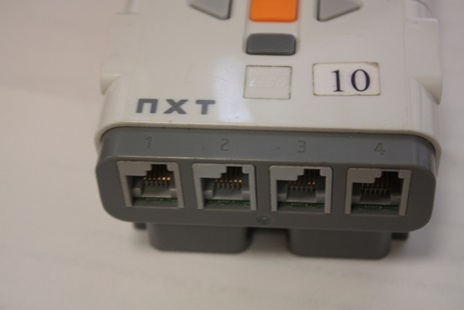
\includegraphics[width=1\linewidth]{chapters/chapter14/images/1}
		\caption{}
		\label{ris:image14x1}
	\end{center}
\end{figure}

Теперь надо рассказать роботу к какому именно выходу и датчик какого типа, мы подключили. Для этого заходим в {\bfseries Robot\(\to\)Motors and Sensors Setup}. Выбираем вкладку Sensors. Выбираем строчку, с номером порта к которому мы подключили датчик. Во вкладке Name (имя) пишем название нашего датчика, то как мы будем обращаться к нему в программе. В принципе имя может быть любым, но разумно называть датчики в соответствии с  тем,  что они меряют, это упрощает чтение кода. Во вкладке Type (тип) выбираем тип датчика. Для датчика расстояния это Sonar.
\clearpage
\begin{figure}[h!]
	\begin{center}
		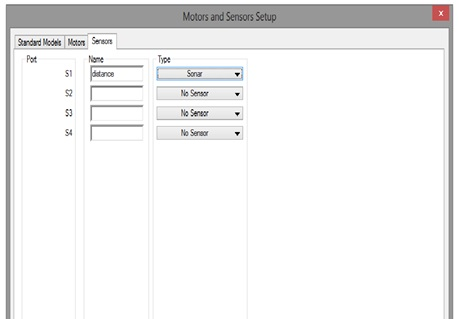
\includegraphics[width=1\linewidth]{chapters/chapter14/images/2}
		\caption{}
		\label{ris:image14x2}
	\end{center}
\end{figure}	

Нажимаем ОК. В результате в программе автоматически сгенерировалась следующая строчка:\\\\
{\programm
	{\slshape\bC{\#pragma~}\bbC{config}}\rC{(\bbC{\slshape{}Sensor},~\rrC{S1},\indent\indent\bbC{\slshape{}distance},\indent\indent\rrC{sensorSONAR})}\\
	\gC{//*!!Code automatically generated by 'ROBOTC' configuration wizard}
}\\\\	

Она и будет означать для компилятора, что на порт 1 подключен сенсор расстояния с именем distance. В соответствии с этой информацией блок будет обрабатывать сигналы с первого порта и превращать их в данные о расстоянии до объекта.

{\slshape В сильных группах можно не только показать алгоритм объявления сенсора, но и подробнее остановиться на причинах. На физическом уровне по кабелю, соединяющему мотор и блок или сенсор и блок, просто идет электрический сигнал: есть напряжение/нет напряжения, величина напряжения. Когда мы управляем мотором~--- на него подается напряжение, чем больше его величина, тем больше мощность, выдаваемая мотором. Что происходит, когда мы подключаем сенсор? В зависимости от внешних условий (освещенности, расстояния до преграды\dots) меняется электрический сигнал, выдаваемый сенсором. Обычно связь примитивная: чем больше расстояние/освещенность/\dots тем больше напряжение на выходе сенсора. Т.е. один и тот же сигнал, к примеру, напряжение в 1 В, на выходе сенсора, может в зависимости от типа сенсора означать совершенно разное: нажата кнопка/в комнате темно/до стола 3 метра. Что бы блок знал, что же в действительности означает получаемый им сигнал мы и указываем тип сенсора. К портам А,В,С по умолчанию можно подключать только моторы, тут проблем не возникает. А при использовании портов 1,2,3,4 необходимо прописать в программе тип сенсора и номер порта.}

Теперь попробуем получить показания с нашего сонара. Для этого существует массив SensorValue[название сенсора],хранящий показания сенсоров. Для датчика расстояния показания возвращаются в сантиметрах до преграды. Если мы напишем: 

\begin{figure}[h!]
	\begin{center}
		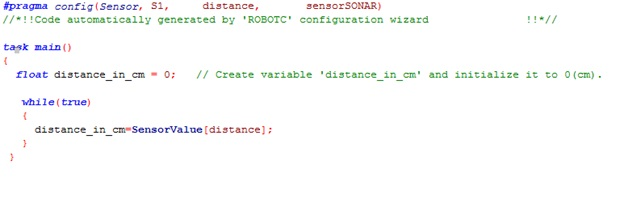
\includegraphics[width=1\linewidth]{chapters/chapter14/images/3}
		\caption{}
		\label{ris:image14x3}
	\end{center}
\end{figure}	

то в переменную distance\_in\_cm  будут непрерывно записываться показания датчика расстояния. Однако пользователю их никак не увидеть. Для начала познакомимся со способом проверить, что на самом деле происходит в программе на каждом шаге, какие значения передаются в какие переменные. Этот метод так же называется отладка по шагам.\\\\

\greenText{Объяснения и принтскрины}\\\\

{\hypertarget{lesson14x3}{\blackBlueText{III. Вывод информации на экран }}}\\\\ 	

\greenText{
	Практикум~---как работать с хелп\\\\	
	Поиск информации по функция display\\\\	
	Практикум~--- написание стандартной программа выводы показаний датчика--проблема--дисретность с wait--сохранение программ-\\\\	
	Что бы не писать каждый раз -библиотеки?
}\\\\

{\hypertarget{lesson14x4}{\blackBlueText{IV. Предобработанные показания датчиков}}}\\\\

Остановимся подробнее на регистрации показаний датчиков. Читатель наверняка заметил, что после задания типа датчика (рис.) в первой строчке программы появляется примерно следующий текст:\\\\

\greenText{sensordefinition}\\\\

\greenText{Первый параметр с скобках означает второй - , третий - , четвертый – тип датчика.}\\\\

В процессе сборки роботов нередко возникает необходимость быстро проверить, что показывает датчик. Например, чтобы проверить, работает ли подключенный датчик, или какие значения он выдает в созданных условиях (цвет поверхности при данном освещении, хорошо ли датчик ультразвуковой сонар определяет расстояния до определенных поверхностей). В таких случаях есть два варианта. Для некоторого количества стандартных датчиков есть возможность посмотреть показания датчиков непосредственно на блоке NXT, не подключая его к компьютеру. Для остальных датчиков необходимо подключение к компьютеру. Рассмотрим подробно оба варианта.

Список датчиков, для которых применим первый вариант, приведен в таблице. 

\begin{center}
	\begin{tabular}[h!]{|c|c|c|}
		\hline
		{Датчик}&{Название в меню}&{Диапазон значений}\\
		\hline
		~ & ~ & ~\\
		\hline
		~ & ~ & ~\\
		\hline
	\end{tabular}
\end{center}

Для регистрации показаний датчика необходимо зайти в пункт меню:\\\\

\greenText{Рисунок}\\\\

И выбрать из списка порт, к которому подключен датчик и тип самого датчика. На экране будут отображаться показания в соответствии с диапазоном выбранного датчика.

Для всех остальных датчиков можно написать простую программу, которая будет выполнять все те же действия, что и встроенная~--- выводить показания датчиков на экран. Пример такой программы:\\\\

\greenText{Программа для снятия показаний датчика}\\\\

Программу необходимо загрузить на блок и запустить. Единственный недостаток такой программы~--- необходимо писать отдельную программу для каждого датчика.

Есть функция, позволяющая определять тип подключенного датчика~--- \greenText{qwerty}. Так что читатель может написать программу, позволяющую выводить на экран блока показания того датчика, который подключен в данный момент. Ее работа основана на определении внутреннего сопротивления датчика. К сожалению, практика показывает, что данная функция часто ошибается.